% Created 2017-02-26 Sun 21:10
% Intended LaTeX compiler: pdflatex
\documentclass[a4paper,11pt]{article}
\usepackage[utf8]{inputenc}
\usepackage[T1]{fontenc}
\usepackage{graphicx}
\usepackage{grffile}
\usepackage{longtable}
\usepackage{wrapfig}
\usepackage{rotating}
\usepackage[normalem]{ulem}
\usepackage{amsmath}
\usepackage{textcomp}
\usepackage{amssymb}
\usepackage{capt-of}
\usepackage{hyperref}
\usepackage[margin=1in]{geometry}
\usepackage{setspace}
\onehalfspacing
\usepackage{parskip}
\usepackage{amsthm}
\usepackage{amsmath}
\usepackage{mathtools}
\usepackage{hyperref}
\usepackage{graphicx}
\usepackage{tabularx}
\usepackage{booktabs}
\hypersetup{colorlinks,citecolor=black,filecolor=black,linkcolor=black,urlcolor=black}
\newtheorem{definition}{Definition}
\newtheorem{theorem}{Theorem}
\newcommand{\rarrowd}[1]{\xrightarrow{\text{ \textit #1 }}}
\DeclareMathOperator*{\plim}{plim}
\newcommand{\plimn}{\plim_{n \rightarrow \infty}}
\setcounter{secnumdepth}{2}
\author{Zheng Tian}
\date{}
\title{Lecture 3: Review of Statistics}
\hypersetup{
 pdfauthor={Zheng Tian},
 pdftitle={Lecture 3: Review of Statistics},
 pdfkeywords={},
 pdfsubject={},
 pdfcreator={Emacs 25.1.1 (Org mode 9.0.3)}, 
 pdflang={English}}
\begin{document}

\maketitle
\setcounter{tocdepth}{2}
\tableofcontents


\section{Introduction}
\label{sec:org2005a62}

Statistics is the science of using data to learn about the world
around us. The key insight of statistics is that one can learn about a
population distribution by selecting a random sample from that
population. Three types of statistical methods are used throughout
econometrics: estimation, hypothesis testing, and confidence
interval. 


\section{Estimation of the Population Mean}
\label{sec:org858c808}

Suppose we draw \(n\) random samples, \(Y_1, \ldots, Y_n\), that are
i.i.d. with the population mean \(\mu_Y\) and the variance \(\sigma^2_Y\),
i.e., \(Y_i \sim IID(\mu_Y, \sigma^2_Y)\) for \(i=1, \ldots, n\). The goal
is to estimate \(\mu_Y\) given these \(n\) samples. A natural way is to
compute the sample average, \(\overline{Y}\). Let see the properties of
\(\overline{Y}\) as an estimator of \(\mu_Y\).

\subsection{Estimators}
\label{sec:orgb0894b8}

An \textbf{estimator} is a function of a sample of data to be drawn randomly
from a population. An \textbf{estimate} is the numerical value of the
estimator when it is actually computed using data from a specific
sample. An estimator is a random variable because of randomness in
selecting the sample, while an estimate is a nonrandom realization of
the estimator. 

Since \(\overline{Y} = (1/n)\sum_{i=1}^n Y_i\), it is an estimator of
\(\mu_Y\). However, \(Y_1\), the first observation, can also be used as an
estimator because it is indeed a function of sample data. As such, we
can have many different estimators of \(\mu_Y\). How can we judge which
estimator is better than another?

We use three criteria to assess an estimator: unbiasedness,
consistency, and efficiency. 

\subsection{Unbiasedness}
\label{sec:org1c1b788}

Let \(\hat{\mu}_Y\) be an estimator of \(\mu_Y\). The estimator
\(\hat{\mu}_Y\) is said to be unbiased if \(\mathrm{E}(\hat{\mu}_Y) =
\mu_Y\), where \(\mathrm{E}(\hat{\mu}_Y)\) is the expectation of the
sampling distribution of \(\hat{\mu}_Y\).

\begin{itemize}
\item \(\overline{Y}\) is an unbiased estimator of \(\mu_Y\). In Lecture 2, we
have already shown that \(\mathrm{E}(\overline{Y}) = \mu_Y\) when \(Y_i
  \sim IID(\mu_Y, \sigma^2_Y)\) for \(i=1, \ldots, n\).
\item \(Y_1\) is also an unbiased estimator because \(\mathrm{E}(Y_1) =
  \mu_Y\) when \(Y_1\) is drawn from \(IID(\mu_Y, \sigma^2_Y)\).
\end{itemize}

\subsection{Consistency}
\label{sec:org555c45f}

\(\hat \mu_Y\) is a consistent estimator of \(\mu_Y\) if \(\hat{\mu}_Y\) is
convergent in probability to \(\mu_Y\). That is, \(\hat{\mu}_Y\) is
consistent if \(\hat{\mu}_Y \xrightarrow{\text{ p }} \mu_Y\) as \(n
\rightarrow \infty\). 

\begin{itemize}
\item \(\overline{Y}\) is a consistent estimator of \(\mu_Y\). The law of large
number ensures that \(\overline{Y} \xrightarrow{\text{ p }} \mu_Y\) is
true when \(Y_i \sim IID(\mu_Y, \sigma^2_Y)\) for \(i=1, \ldots, n\), and \(\sigma^2_Y <
  \infty\).

\item However, we cannot assess the consistency for \(Y_1\) because it cannot
be written as the form of an average.
\end{itemize}

\subsection{Variance and efficiency}
\label{sec:org77a6d27}

When both \(\tilde{\mu}_Y\) and \(\hat{\mu}_Y\) are two unbiased
estimators of \(\mu_Y\), we choose the estimator with the tightest
sampling distribution, which means the smallest variance. Thus,
\(\hat{\mu}_Y\) is said to be more efficient than \(\tilde{\mu}_Y\) if
\(\mathrm{Var}(\hat{\mu}_Y) < \mathrm{Var}(\tilde{\mu}_Y)\).

In words, \(\hat{\mu}_Y\) is more efficient than \(\tilde{\mu}_Y\)
because \(\hat{\mu}_Y\) uses the information in the data more
efficiently than does \(\tilde{\mu}_Y\). 

In Lecture 2, we compute the variance of \(\overline{Y}\) to be
\(\sigma^2_Y / n\) when \(Y_i \sim IID(\mu_Y, \sigma^2_Y)\). The variance
of \(Y_1\) is \(\sigma^2_Y\). When \(n > 1\), \(\overline{Y}\) is more
efficient than \(Y_1\). 

\subsection{\(\overline{Y}\) is the best linear unbiased estimator (BLUE)}
\label{sec:org99c9ae6}

In fact, \(\overline{Y}\) happens to be the best linear unbiased
estimator (BLUE). It means that among all linear unbiased estimator,
\(\overline{Y}\) has the smallest variance. 

A linear estimator of \(\mu_Y\) is a weighted average of \(Y_1, \ldots,
Y_n\), written as
\[ \tilde{\mu}_Y = \frac{1}{n} \sum_{i=1}^n \alpha_i Y_i \]
where \(\alpha_1, \ldots, \alpha_n\) are nonrandom constants. 

If \(\tilde{\mu}_Y\) is another unbiased estimator of \(\mu_Y\), then we
always have \(\mathrm{Var}(\overline{Y}) \leq
\mathrm{Var}(\tilde{\mu}_Y)\), and the equality holds only if
\(\tilde{\mu}_Y = \overline{Y}\). It means that \(\overline{Y}\) is BLUE.

\subsubsection*{The proof of \(\mathrm{Var(\overline{Y})} \leq \mathrm{Var}(\tilde{\mu}_Y)\)}
\label{sec:orge32ac84}

That \(\tilde{\mu}_Y\) is an unbiased estimator of \(\mu_Y\) means that
\[\mu_Y = \mathrm{E}(\tilde{\mu}_Y) = \mathrm{E}\left( \frac{1}{n} \sum_{i=1}^n \alpha_i
Y_i \right) = \frac{1}{n} \mu_Y \sum_{i=1}^n \alpha_i \]
which requires \(\frac{1}{n} \sum_{i=1}^n \alpha_i = 1\). 

We know the variance of \(\mathrm{Var}(\overline{Y})\) is
\(\sigma^2_Y / n\), and the variance of \(\tilde{\mu}_Y\) can be computed as
\begin{equation*}
\mathrm{Var}(\tilde{\mu}_Y) = \frac{1}{n^2} \sum_{i=1}^n \alpha_i^2 \mathrm{Var}(Y_i) = \frac{\sigma^2_Y}{n^2} \sum_{i=1}^n \alpha_i^2 
\end{equation*}
So, to prove \(\mathrm{Var}(\tilde{\mu}_Y) \geq
\mathrm{Var}(\overline{Y})\), we only need to show
\(\frac{1}{n}\sum_{i=1}^n \alpha_i^2 \geq 1\).  

\[
\frac{1}{n}\sum_{i=1}^n \alpha_i^2 = \frac{1}{n} \sum_{i=1}^n
(\alpha_i^2 - 2\alpha_i + 1) + \frac{1}{n}\sum_{i=1}^n 2\alpha_i - 1 =
\frac{1}{n} \sum_{i=1}^n (\alpha_i - 1)^2 + 1 \geq 1 \] 

The second equality holds because \(\frac{1}{n} \sum_{i=1}^n \alpha_i =
1\).  And \(\mathrm{Var}(\tilde{\mu}_Y) = \mathrm{Var}(\overline{Y})\)
only if \(\alpha_i = 1\) for all \(i=1, \ldots, n\), which is equivalent
to \(\tilde{\mu}_Y = \overline{Y}\).

\subsection{\(\overline{Y}\) is the least squares estimator of \(\mu_Y\)}
\label{sec:org70f0d1f}

Consider the following model
  \[ Y_i = \alpha + u_i \text{ for } i = 1, 2, \ldots, n \]
where \(\alpha\) is a nonrandom intercept to be estimated, \(u_i\) is
the error term, which is a random variable with \(\mathrm{E}(u_i) = 0\). 

Thus, we have \(E(Y_i) = \alpha = \mu_Y\). That means \(\alpha\) is the
mean of \(Y_i\), and an estimator for \(\alpha\) is just an estimator for
\(\mu_Y\). \(u_i\) can be seen as the error of predicting \(Y_i\) with
\(\alpha\) for each \(i\), and we use \(\sum_{i=1}^n (Y_i - \alpha)^2\) to
measure the total prediction errors. A natural choice of an estimator
of \(\alpha\) is the one that minimizes this sum of squared errors. 

The least squares estimator of \(\mu_Y\) (or \(\alpha\)) is obtained by
solving the following problem
  \[ \operatorname*{min}_a\: \sum_{i=1}^n (Y_i - a)^2 \]
The solution of this minimization problem is just \(a = \overline{Y}\). 

\subsubsection*{The proof for \(\overline{Y}\) is the least square estimator}
\label{sec:org671d556}

The first order condition for the minimization problem is
\begin{equation*}
  \frac{d}{da}\sum_{i=1}^n (Y_i - a)^2 = -2\sum_{i=1}^n(Y_i - a) = -2\sum_{i=1}^n Y_i+ 2n a = 0      
\end{equation*}
Solving the equation for \(a\), we get \(a = 1/n\sum_{i=1}^n Y_i = \overline{Y}\).


\section{Hypothesis Tests Concerning the Population Mean}
\label{sec:orga3b7dd9}

\subsection{Null and alternative hypotheses}
\label{sec:orge9fd355}

With the estimate of the population mean, we can test some hypotheses
regarding the mean. Hypothesis testing is thus to make a provisional
decision based on the evidence at hand on. We first set up a
hypothesis to be tested, called the \textbf{null hypothesis}, and a second
hypothesis called the \textbf{alternative hypothesis} that holds if the null
does not. 

In this lecture, we focus on the hypothesis of the population mean,
\(\mathrm{E}(Y)\), taking on a specific value, \(\mu_{Y,0}\). So the null
hypothesis, denoted as \(H_0\), is
\[ H_0: E(Y) = \mu_{Y,0}  \]

The alternative hypothesis, denoted as \(H_1\), can be either two-sided,
i.e., \(H_1: E(Y) \neq \mu_{Y,0}\), or one-sided, i.e., \(H_1: E(Y) >
\mu_{Y,0}\), depending on the question of interest. 

One thing should be kept in mind is that we usually do not say "accept
the null hypothesis" when the hypothesis test is in favor of the null,
but say "fail to reject the null". That means, that given the sample
data at hand, we do not have sufficient evidence to prove the null
hypothesis is false, but it is likely that the null would be rejected
given another set of samples.

\subsection{Test statistics}
\label{sec:orgf6ba2bd}

Upon setting up the hypotheses to be tested, we need test statistics to be
used in the test. In the case of testing the population mean,
\(\mathrm{E}(Y)\), we find two test statistics in two different
situations: the z-statistic when \(\sigma_Y\) is known and the
t-statistic when \(\sigma_Y\) is unknown

\subsubsection*{The z-statistic when \(\sigma_Y\) is known}
\label{sec:orgd053220}

We know that when \(Y_i \sim IID(\mu_Y, \sigma^2_Y)\) for \(i=1, \ldots,
n\), \(E(\overline{Y}) = \mu_Y\) and
\(\mathrm{Var}(\overline{Y}) = \sigma^2_{\overline{Y}} = \sigma^2_Y /
n\). In the null hypothesis, we specify \(\mu_Y = \mu_{Y,0}\). So given
that \(\sigma_Y\) is known, the
z-statistic is computed as 
\[ z = \frac{\overline{Y} -
  \mu_{Y,0}}{\sigma_{\overline{Y}}} = \frac{\overline{Y} -
  \mu_{Y,0}}{\sigma_Y/\sqrt{n}} \]
As \(n \rightarrow \infty\), by the central limit theorem, we know \(z
\xrightarrow{\text{ d }} N(0, 1)\). 

\subsubsection*{The t-statistic when \(\sigma_Y\) is unknown}
\label{sec:org4317364}

Of course, \(\sigma_Y\) is the standard deviation of the population
variance that is usually unknown. So we need to replace \(\sigma_Y\)
with its estimator. 

\begin{itemize}
\item The sample variance and standard deviation
\label{sec:org482d3ff}

The \textbf{sample variance} \(s^2_Y\) is is an estimator of the population
variance \(\sigma^2_Y\), which is computed as
  \[ s^2_Y = \frac{1}{n-1}\sum^n_{i=1} (Y_i - \overline{Y})^2 \]
The \textbf{sample standard deviation}, \(s_Y\), is the square root of \(s^2_Y\). 

We can prove that the sample variance, \(s^2_Y\), is a consistent estimator of the
population variance, that is, as \(n \rightarrow \infty\), \(s^2_Y
\xrightarrow{\text{ p }} \sigma^2_Y\). (See the proof in
Appendix 3.3.)

\item The standard error of \(\overline{Y}\)
\label{sec:orgbbf467c}

The standard error of \(\overline{Y}\), denoted as \(SE(\overline{Y})\) or
\(\hat{\sigma}_{\overline{Y}}\), is an estimator of the standard
deviation of \(\overline{Y}\),
\(\sigma_{\overline{Y}}=\sigma_Y/\sqrt{n}\), with \(s_Y\) replacing
\(\sigma_Y\). 
\[ SE(\overline{Y}) = \hat{\sigma}_{\overline{Y}} =
\frac{s_Y}{\sqrt{n}} \]

\item The t-statistic
\label{sec:orgc67635c}

When \(\sigma_Y\) is unknown, by replacing \(\sigma_Y\) with \(s_Y\), we
have the t statistic 
  \[ t = \frac{\overline{Y} - \mu_{Y,0}}{SE(\overline{Y})} =
  \frac{\overline{Y} - \mu_{Y,0}}{s_Y/\sqrt{n}} \] 

\begin{itemize}
\item The asymptotic distribution of the t statistic is \(N(0, 1)\) because
\(s_Y\) is a consistent estimator of \(\sigma_Y\).

\item When \(Y_i\) for \(i=1, \ldots, n\) are i.i.d. from \(N(\mu_Y,
  \sigma_Y^{2})\), we can show that the exact distribution for the
Student t
statistic is the Student t distribution with \((n-1)\) degrees of
freedom. That is
\[ t \sim t(n-1)  \]
(See Section 3.6, Page 129, in the textbook for a discussion about the
reason for t has a t distribution with \(n-1\) degree of freedom.)
\end{itemize}
\end{itemize}

\subsection{Hypothesis testing with a pre-specified significance level}
\label{sec:org41615d4}

With the null and alternative hypotheses being the goal of the test
and test statistics being the tools, we need a rule to make a
judgment: When can we reject (or fail to reject) the null hypothesis
if the test statistic takes on what values? To do so, we need to first
define some concepts. 

\subsubsection*{Type I and type II errors}
\label{sec:org734fad6}

A statistical hypothesis test can make two types of mistakes:
\begin{itemize}
\item \textbf{Type I error}. The null hypothesis is rejected when in fact it is
true.
\item \textbf{Type II error}. The null hypothesis is not rejected when in fact it
is false.
\end{itemize}

The probability of making a type I error is easier to be identified
and controlled than that of a type II error. So the commonly practiced
rule of judging a hypothesis test concerns avoiding the type I error.

\subsubsection*{The significance level and the critical value}
\label{sec:org4219d5c}

\begin{itemize}
\item The \textbf{significance level} is the pre-specified probability of type I error.
Usually, we set the significance level to be \(\alpha = 0.05, 0.10,
  \text{ or } 0.01\).

\item The \textbf{critical value}, denoted as \(c_{\alpha}\), is the value of the test statistic for which
the test rejects the null hypothesis at the given significance
level. The \(N(0, 1)\) critical value for a two-sided test with a 5\%
significance level is 1.96.

\item The \textbf{rejection rule}.  For a two-sided test, we reject the null
hypothesis when \(|z^{act}| > c_{\alpha}\).

\item The rejection rule is easier to be understood with the rejection and
acceptance region, as shown in Figure \ref{fig:orgc6283cd}. The
\textbf{rejection region} is the set of values of the test statistic for
which the test rejects the null, and the \textbf{acceptance region} is the
vice.

\begin{figure}[htbp]
\centering
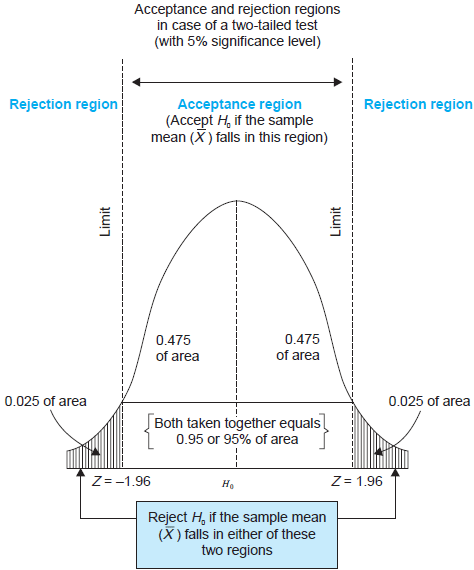
\includegraphics[width=0.7\textwidth]{figure/fig9_1.png}
\caption{\label{fig:orgc6283cd}
An illustration of a two-sided test}
\end{figure}
\end{itemize}

\subsubsection*{The power and the size of the test}
\label{sec:orgdcb6f6f}

\begin{itemize}
\item The \textbf{size} of the test is the probability that the test actually
incorrectly rejects the null hypothesis when it is true. That is,
the size of the test is just the significance level.

\item The \textbf{power} of the test is the probability that the test correctly
rejects the null when the alternative is true. That is,
\(\text{power} = 1 - \mathrm{Pr}(\text{type II error})\)
\end{itemize}

\subsection{The p-value}
\label{sec:org66f4208}

The \textbf{p-value}, also called the \textbf{significance probability}, is the
probability of drawing a statistic at least as adverse to the null
hypothesis as the one you actually computed in your sample, assuming
the null hypothesis is correct.

The p-value provides more information than the significance level. In
fact, the p-value is also named the marginal significance level, which
the smallest significance level at which you can reject the null
hypothesis. The rejection rule of rejecting the null is then the
\(\text{p-value} < \alpha\).

Mathematically, the p-value is computed as

\begin{equation*}
p\text{-value} = 
\begin{cases}
\mathrm{Pr}_{H_0}\left(|z| > |z^{act}|\right)=2\Phi(-|z^{act}|) \text{ when } \sigma_Y \text{ is known} \\
\mathrm{Pr}_{H_0}\left(|t| > |t^{act}|\right)=2\Phi(-|t^{act}|) \text{ when } \sigma_Y \text{ is unknown}
\end{cases}
\end{equation*}

\subsection{One-sided alternatives}
\label{sec:org9095f7b}

For a one-sided alternative hypothesis, \(H_1: \mathrm{E}(Y) >
\mu_{Y,0}\), we can compute the p-value as
\[ p\text{-value} = \mathrm{Pr}_{H_0}(t > t^{act}) = 1 - \Phi(t^{act}) \]

The \(N(0, 1)\) critical value for a one-sided test with a 5\%
significance level is 1.64. The rejection region for this test is all
values of the t-statistic exceeding 1.64. 


\section{Confidence Intervals for the Population Mean}
\label{sec:org88122a3}

\subsection{Definitions}
\label{sec:org1f34945}

\begin{itemize}
\item A \textbf{confidence set} is the set of values that contains the true
population mean \(\mu_Y\) with a certain prespecified probability.

\item A \textbf{confidence level} is the prespecified probability that \(\mu_Y\) is
contained in the confidence set. \(\text{confidence level} = 1 -
  \text{significance level}\).

\item A \textbf{confidence interval} is the confidence set when it is an
interval.

\item In the case of a two-sided test for \(\mu_Y\), we say that a 95\%
confidence interval is an interval constructed so that it contains
the true value of \(\mu_Y\) in 95\% of all possible random samples.
\end{itemize}

\subsection{Constructing a confidence interval based on the t statistic}
\label{sec:org76e9eee}

\begin{itemize}
\item Step 1: we compute the t statistic for the two-sided test
\[ t = \frac{\overline{Y} - \mu_{Y,0}}{SE(\overline{Y})}
   \xrightarrow{\text{ d }} N(0, 1) \]

\item Step 2: we know that we fail to reject the null at the 5\% level if \(|t| <
  1.96\).

\item Step 3: we plug in the definition of \(t\) and solving for \(|t| \leq 1.96\), we
get
\begin{align*}
-1.96 & \leq \frac{\overline{Y} - \mu_{Y,0}}{SE(\overline{Y})} \leq 1.96 \\
\overline{Y} - 1.96 SE(\overline{Y}) & \leq \mu_{Y,0} \leq \overline{Y} + 1.96 SE(\overline{Y})
\end{align*}

Thus, the 95\% confidence interval two-sided confidence interval for
\(\mu_Y\) is 
\[ \{ \overline{Y} \pm 1.96 SE(\overline{Y}) \} \]
\end{itemize}

Similarly, we can get 
\begin{itemize}
\item 90\% confidence interval for \(\mu_Y = \{ \overline{Y} \pm 1.64
  SE(\overline{Y}) \}\)
\item 99\% confidence interval for \(\mu_Y = \{ \overline{Y} \pm 2.58
  SE(\overline{Y}) \}\)
\end{itemize}


\section{Comparing Means from Different Populations}
\label{sec:org7a34210}

\subsection{Hypothesis tests for the difference between two means}
\label{sec:orgd6c6e9d}

Now we extend hypothesis testing involving one population mean to that
regarding comparison between two population means. Say, the difference
in earnings between male college graduates and female college
graduates. The basic ideas and procedure in this test is the same as
for testing the single population mean. 

Let \(Y_{m, i}\) for \(i=1, \ldots, n_m\) be \(n_m\) i.i.d. samples from the
population of earnings of male college graduate, i.e., 
\[ Y_{m,i} \sim IID(\mu_m, \sigma^2_m)  \text{ for } i=1,\ldots,n_m \]
and \(Y_{w, j}\) for
\(j=1, \ldots, n_w\) be \(n_w\) i.i.d. samples from the population of
earnings of female college graduate, i.e.,
\[ Y_{w,j} \sim IID(\mu_w, \sigma^2_w)  \text{ for } j=1,\ldots,n_w \]
Also, we assume that \(Y_{m,i}\) and \(Y_{w,j}\) are independent. 

The hypothesis to be tested is whether the mean earnings for the male and
female graduates differ by a certain amount, that is, 
\[ H_0: \mu_m - \mu_w = d_0,\; \text{ vs. }\: H_1: \mu_m - \mu_w \neq d_0 \]

As in the test for the single population mean, we can take the
following steps to test the difference in two population means:
\begin{enumerate}
\item Calculate the sample average earnings: \(\overline{Y}_m\) for the
male and \(\overline{Y}_w\) for the female. \(\overline{Y}_m\) and
\(\overline{Y}_w\) are the unbiased estimators for \(\mu_m\) and
\(\mu_w\), respectively.

As \(n_m\) and \(n_w\) get large, we know \(\overline{Y}_m
   \xrightarrow{\text{ d }} N(\mu_Y, \sigma^2_m/n_m)\), and
\(\overline{Y}_w \xrightarrow{d} N(\mu_w, \sigma^2_w / n_w)\). 

Given that \(\overline{Y}_m - \overline{Y}_w\) is a linear function
of \(\overline{Y}_m\) and \(\overline{Y}_w\), and \(Y_{m,i}\) and
\(Y_{w,j}\) are independent, we know that 
\[(\overline{Y}_m - \overline{Y}_w) \xrightarrow{d} N(\mu_m -
   \mu_w,\; \frac{\sigma^2_m}{n_m} + \frac{\sigma^2_w}{n_w}) \]

\item When \(\sigma^2_m\) and \(\sigma^2_w\) are known, we use the z statistic
\[ z = \frac{(\overline{Y}_m - \overline{Y}_w) - d_0}{\left(
   \frac{\sigma^2_m}{n_m} + \frac{\sigma^2_w}{n_w} \right)^{1/2}}
   \xrightarrow{\text{ d }} N(0, 1) \]

When \(\sigma^2_m\) and \(\sigma^2_w\) are unknown, we the t
statistic
\[ t = \frac{(\overline{Y}_m - \overline{Y}_w) -
   d_0}{SE(\overline{Y}_m - \overline{Y}_w)} \xrightarrow{\text{ d }}
   N(0, 1) \] 
where
\begin{gather*}
SE(\overline{Y}_m - \overline{Y}_w) = \left(\frac{s^2_m}{n_m} + \frac{s^2_w}{n_w} \right)^{1/2} \\
s^2_m = \frac{1}{n_m-1}\sum^{n_m}_{i=1}(Y_{m,i} - \overline{Y}_m)^2 \\
s^2_w = \frac{1}{n_w-1}\sum^{n_w}_{i=1}(Y_{w,i} - \overline{Y}_w)^2
\end{gather*}

\item Calculate the p value: The p value for the two-sided test is calculated as 
\[ p\text{-value} = 2\Phi(-|t|) \]

For a two-sided test at the 5\% significant level, we can reject
the null hypothesis when the p value is less than 5\%, or,
equivalently, when \(|t| > 1.96\).
\end{enumerate}

\subsection{Confidence intervals for the difference between two means}
\label{sec:org2f482f7}

The 95\% confidence interval can be constructed as usual based on the t
statistic we have computed above. That is, the 95\% confidence interval
for \(d = \mu_m - \mu_w\) is
\[ (\overline{Y}_m - \overline{Y}_w) \pm 1.96SE(\overline{Y}_m -
\overline{Y}_w) \]

\subsection{Differences-of-Means Estimation of Causal Effects Using Experimental Data}
\label{sec:org90d196b}

The difference-of-means estimation and hypothesis test can be used in
estimation of causal effect in ideal randomized controlled
experiments (RCE). 

We define the outcome of a RCE to be \(Y\) and the binary treatment
variable to be \(X\), \(X=1\) for the treatment group and \(X=0\) for the
control group. Then the causal effect of the treatment can be
conveniently expressed as the difference in the conditional
expectation, 
\[ E(Y \mid X=1) - E(Y \mid X=0)  \]

We can consider the treatment group and the control group to represent two
independent population. Then, we can use the estimation and hypothesis
test regarding the difference between two population means to examine
the causal effect. 


\section{Scatterplots, the Sample Covariance, and the Sample Correlation}
\label{sec:org695e0e6}

\subsection{Scatterplots}
\label{sec:orga03f956}

Before a formal statistical study, we often first do some exploratory
analysis. Drawing graphs is an important aspect of exploratory data
analysis to visualize the patterns of the variables of
interests. 

A \textbf{scatterplot} is a plot of \(n\) observations on \(X_i\) and \(Y_i\), in
which each observation is represented by the point \((X_i,
Y_i)\). Figure \ref{fig:org01d3167} is the scatterplot between test scores and the
student-teacher ratios in the example of California school districts. 

\begin{figure}[htbp]
\centering
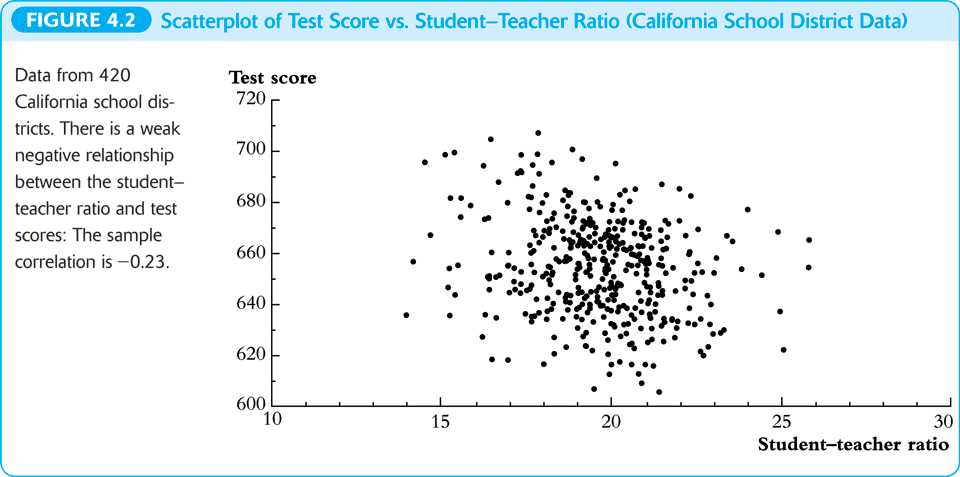
\includegraphics[width=0.9\textwidth]{figure/fig-4-2.png}
\caption{\label{fig:org01d3167}
The scatterplot between test scores and student-teacher ratios}
\end{figure}

\subsection{Sample covariance and correlation}
\label{sec:orgeba5041}

The population covariance and correlation measure the relation between
two random variables \(X\) and \(Y\) in their population joint probability
distribution. Since they are typically unknown, we use the \textbf{sample
covariance} and the \textbf{sample correlation coefficient} as their
estimators. 

\subsubsection*{Sample covariance}
\label{sec:orgd877752}

The \textbf{sample covariance}, denoted as \(s_{XY}\), is
\[ s_{XY} = \frac{1}{n-1}\sum^n_{i=1}(X_i - \overline{X})(Y_i -
\overline{Y}) \]

\subsubsection*{Sample correlation}
\label{sec:orgb7c0c58}

The \textbf{sample correlation coefficient}, denoted as \(r_{XY}\), is
\[ r_{XY} = \frac{s_{XY}}{s_X s_Y} \]
and we have \(|r_{XY}| \leq 1\). 

\subsubsection*{Consistency of the sample covariance and correlation}
\label{sec:org8f46f3b}

If \((X_i,\, Y_i)\) are i.i.d. and \(X_i\) and \(Y_i\) have finite fourth
moments, then
\[ s_{XY} \xrightarrow{\text{ p }} \sigma_{XY} \text{ and } r_{XY}
\xrightarrow{\text{ p } } \rho_{XY} \]

\subsubsection*{The correlation coefficient measures the linear association}
\label{sec:org53f401f}

We should emphasize that the correlation coefficient is a measure of
linear association between \(X\) and \(Y\). There could be a relationship
with zero correlation coefficient, but is in fact nonlinear, as shown
in Figure \ref{fig:orgcbe0200}. 

\begin{figure}[htbp]
\centering
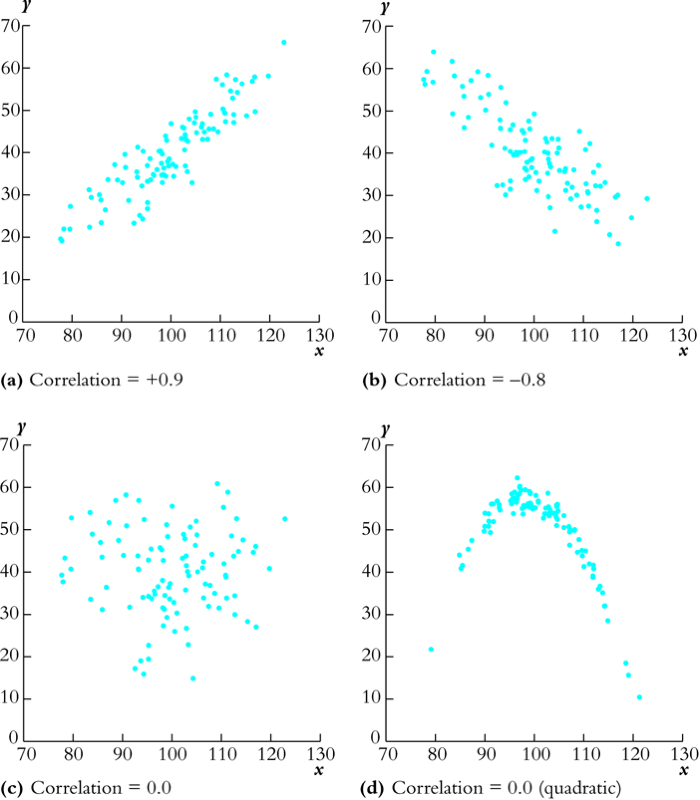
\includegraphics[width=0.6\textwidth]{figure/fig-3-3.png}
\caption{\label{fig:orgcbe0200}
Scatterplots for four hypothetical data sets}
\end{figure}
\end{document}